\section{How should macroprudential policy respond to risks?}
\subsection{Macroprudential policy uses}
Prior to the 2008 Great Recession, macroprudential regulation remained largely underdeveloped. The policy primarily focused on microprudential approaches and operated under the assumption that strong individual institutions would result in a stable financial system \citep{galati2013}. However, systemic risks related to leverage and bank interconnectedness remained high. The financial crisis revealed these vulnerabilities, prompting a shift in policymakers' focus from micro-level concerns to broader, macroprudential considerations. The Central Bank of Armenia (CBA) was no exception, implementing a series of tightening measures in the aftermath of the crisis.

\autoref{fig:arm_MPI_actions} illustrates the evolution of tightening and loosening macroprudential measures in Armenia. Following the 2008 Great Recession, most regulatory changes focused on capital and asset risk weights. Indirect loosening measures were also used. In 2016, the risk weights for mortgage loans denominated in local currency that met specific criteria were reduced from 50\% to 35\%. Additionally, in February of that year, the risk weights for correspondent accounts, set at 20\% for AMD and 30\% for FX, were extended to demand deposits of banks with maturities of up to three months. These regulations effectively lowered banks' risk-weighted assets (RWA) relative to their equity, making it easier to meet capital requirements.
\begin{figure}
	\centering 
	
\includegraphics[width=0.45\textwidth, angle=0]{Figures/arm_MPI_actions.png}	
	\caption{Use of macroprudential policy in Armenia. The Y-axis shows the number of policy actions taken.} 
	\label{fig:arm_MPI_actions}%
\end{figure}

In 2020, the CBA adopted a more accommodative stance in response to the economic impacts of the Covid-19 pandemic. Specifically, funds received from state support programs were exempted from reserve requirements, providing relief to banks during the economic downturn. This marked a temporary shift toward loosening regulatory requirements to support financial stability during the crisis.

In April 2022, the CBA implemented currency-based loan-to-value (LTV) caps, setting a maximum LTV ratio of 90\% for real estate loans in AMD and 70\% for those in FX. Lastly, although the minimum CAR was reduced from 12\% to 11\%, other capital-based measures increased. The CCyB was raised from 1\% (effective from May 2023) to 1.5\% (effective from August 2023), the buffer for systemically important financial institutions (SIFIs) increased from 1\% to 1.5\%, and the capital conservation buffer (CCoB) was raised from 1.5\% to 2\%. Collectively, these measures resulted in a net tightening of the macroprudential policy.

To analyze the impact of these policies we compare the GDP growth distribution of Armenia one year after tightening actions, as shown in \autoref{fig:arm_MPI_tightening_gdp_dist}. The comparison distinguishes between stable and crisis periods. The results indicate that when tightening actions are not followed by a crisis, there is little effect on the left tail of the distribution. However, these actions tend to reduce the right tail, suggesting that they may limit the potential for excessive economic growth. Meanwhile, when a tightening action is followed by a crisis, the distribution shows a less severe left tail. This suggests that tightening policies may mitigate the severity of economic downturns. Finally, the right tail remains relatively unaffected.

To continue our analysis of the evolution of macroprudential policy, in \autoref{fig:panel_MP_use_TL} we investigate the tightening and loosening measures used in the other 40 countries of our study. We observe an active use of loosening measures during the 2008-2009 crisis, in 2012 during the European debt crisis, and during the 2020 Covid-19 pandemic. We also observe an increase in the number of tightening measures starting 2015. \autoref{fig:panel_MP_action_decomp} also delves deeper into the specific measures used over time. In 2009 and 2012 the majority of loosening measures were implemented thought reserve requirements, while in 2020 a much wider array of tools was available for the policymakers, including capital and liquidity-based measures, loan loss provisions (LLPs), LTV measures, and many others \citep{mack2021}. Lastly, the increase in tightening measures in 2015 was primarily driven by the introduction of capital conservation buffers and liquidity measures such as liquidity coverage ratio (LCR), liquid asset ratio (LAR), and net stable funding ratio (NSFR).
\begin{figure}
	\centering 
	
\includegraphics[width=0.45\textwidth, angle=0]{Figures/panel_MP_use_TL.png}	
	\caption{Use of macroprudential policy in 41 countries. The Y-axis shows the number of policy actions taken.} 
	\label{fig:panel_MP_use_TL}%
\end{figure}
\begin{figure*}
	\centering 
	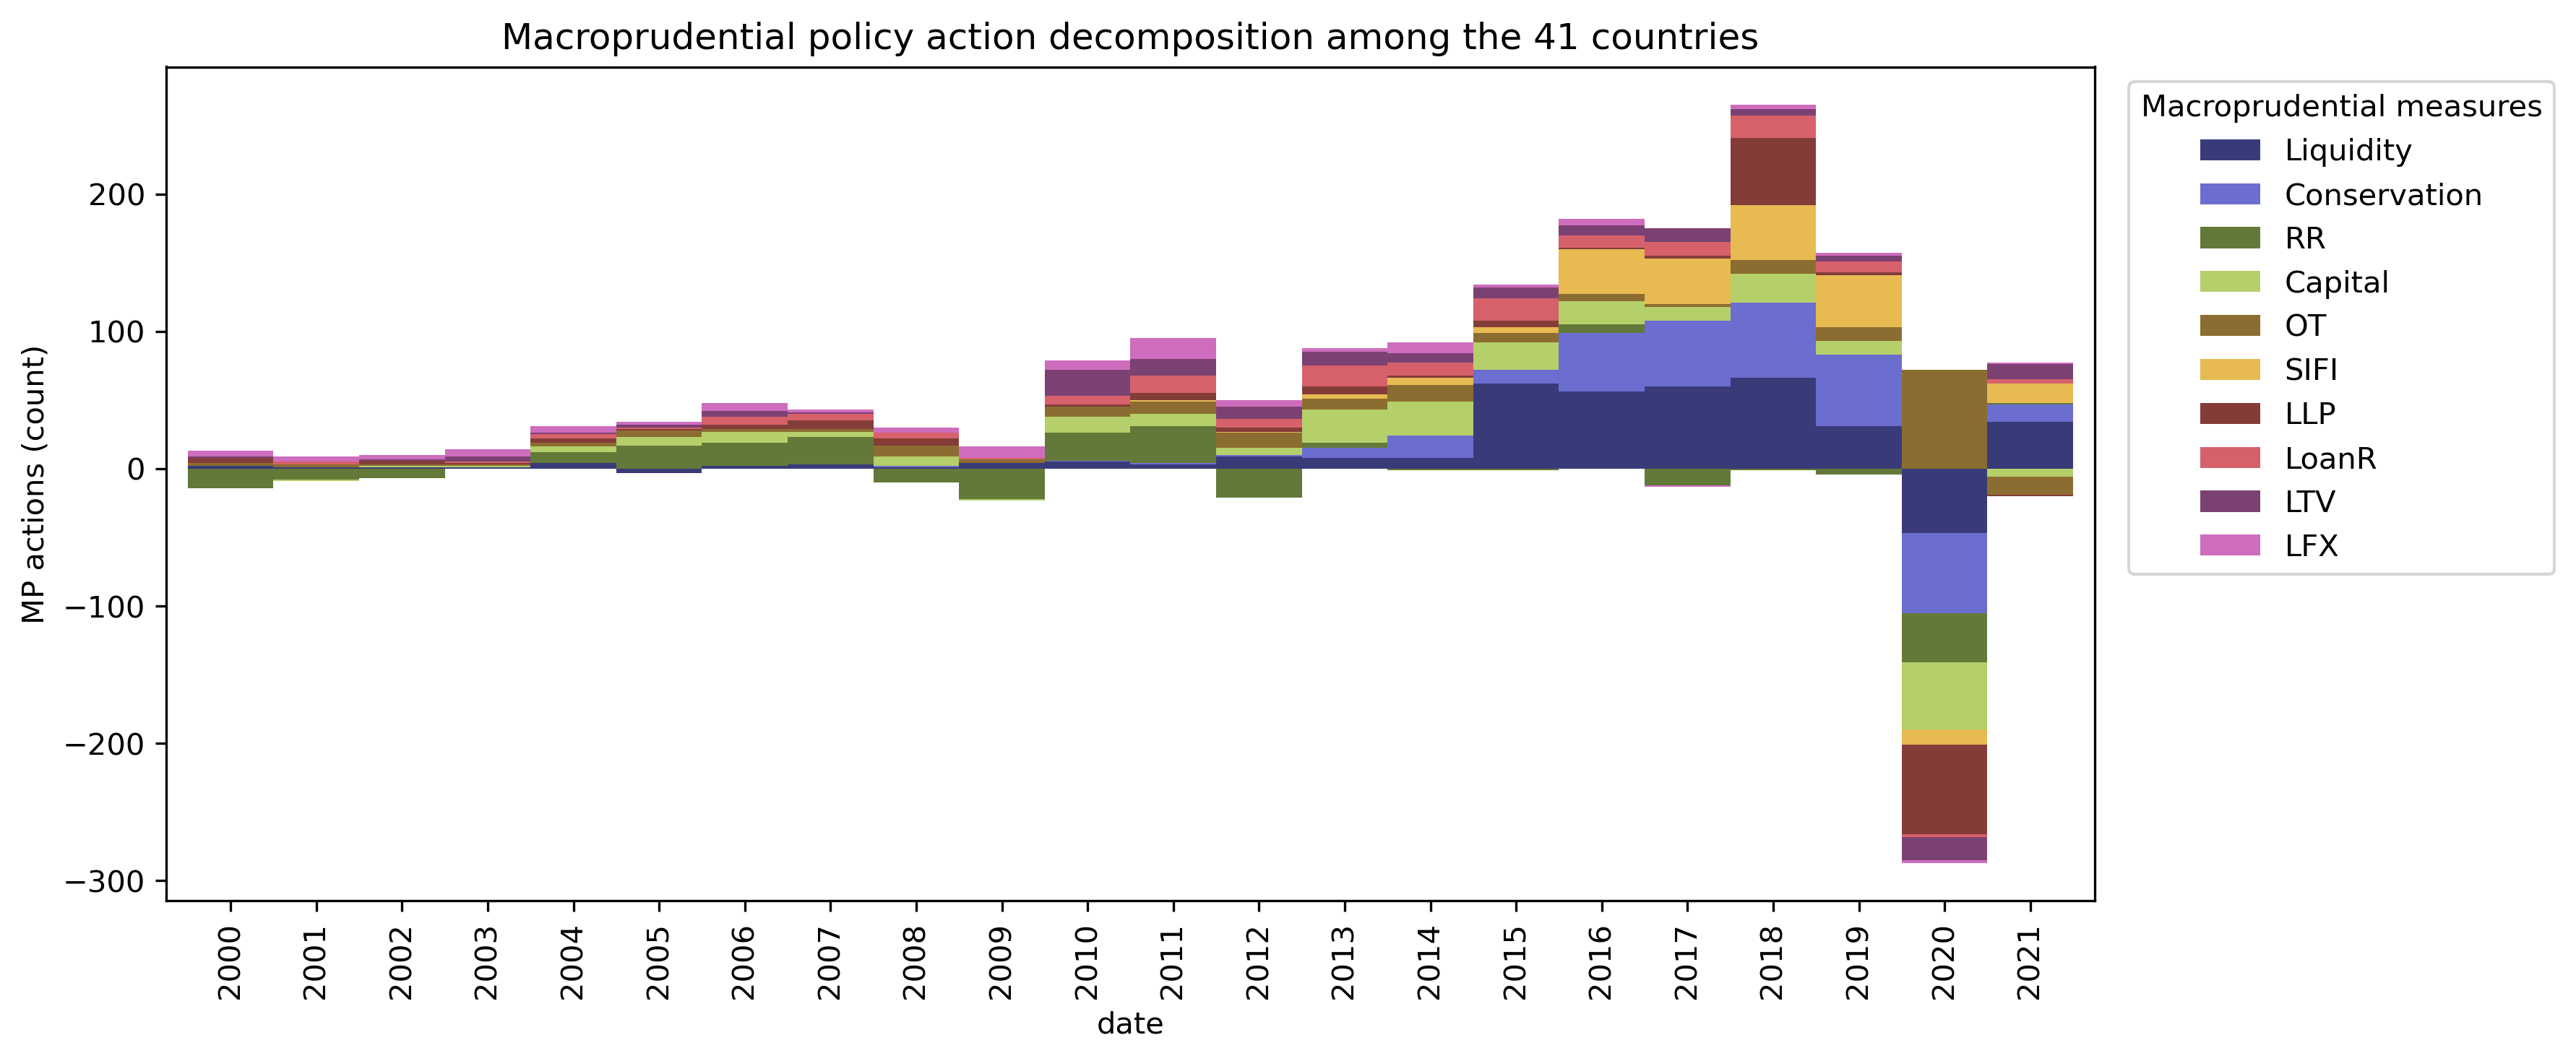
\includegraphics[width=1\textwidth, angle=0]{Figures/panel_MP_action_decomp.png}	
	\caption{Use of macroprudential policy in 41 countries and decomposition of macroprudential measures. The Y-axis shows the net number of tightening vs loosening policy actions taken.} 
	\label{fig:panel_MP_action_decomp}%
\end{figure*}

We examine the impact of macroprudential policy on the GDP growth distribution of the 41 countries in \autoref{fig:panel_MP_use_before_crisis}. During the crisis period the major difference is observed on the right tail of the distribution, which may imply faster recovery \citep{stojkov2020}. The difference becomes more significant when examining the recovery period. Countries that had implemented prior tightening measures had higher GDP growth in this period.

\subsection{Materialization of risks}
Macroprudential policy affects the GDP growth distribution by regulating the buildup of systemic risks. These vulnerabilities tend to accumulate during periods characterized by rising asset prices and low market volatility. In such environments, the ease of borrowing encourages economic agents to increase leverage. These conditions reduce the incentives of financial intermediaries to manage liquidity and solvency risks while simultaneously expanding their lending capacity and risk appetite. Consequently, this leads to negative externalities, manifesting as “increased leverage, mismatches of maturity and financial positions, growing indebtedness, reduced debt servicing capacity, and other balance sheet weaknesses” \citep{imf_gar_2019}. During periods of financial stress, banks reduce lending and engage in deleveraging, which further exacerbates the decline in asset prices. Ultimately, these exposures contribute to deeper, more prolonged, and severe economic downturns \citep{Cardarelli_2011}.

In \autoref{fig:theory_gdp_unconditional}, we present the unconditional GDP growth distribution of Armenia. The dotted lines represent the median and the 10th percentile (or tail) of the distribution. The difference between the median and the tail, referred to as the “distance-to-tail,” reflects the unconditional risks faced by the financial system. This metric captures not only the direct impact of potential crises but also the amplifying effects of systemic risks. In the case of Armenia, a crisis, defined as the worst 10\% of possible outcomes, could reduce GDP growth by up to 12.4\%.
\begin{figure}
	\centering 
	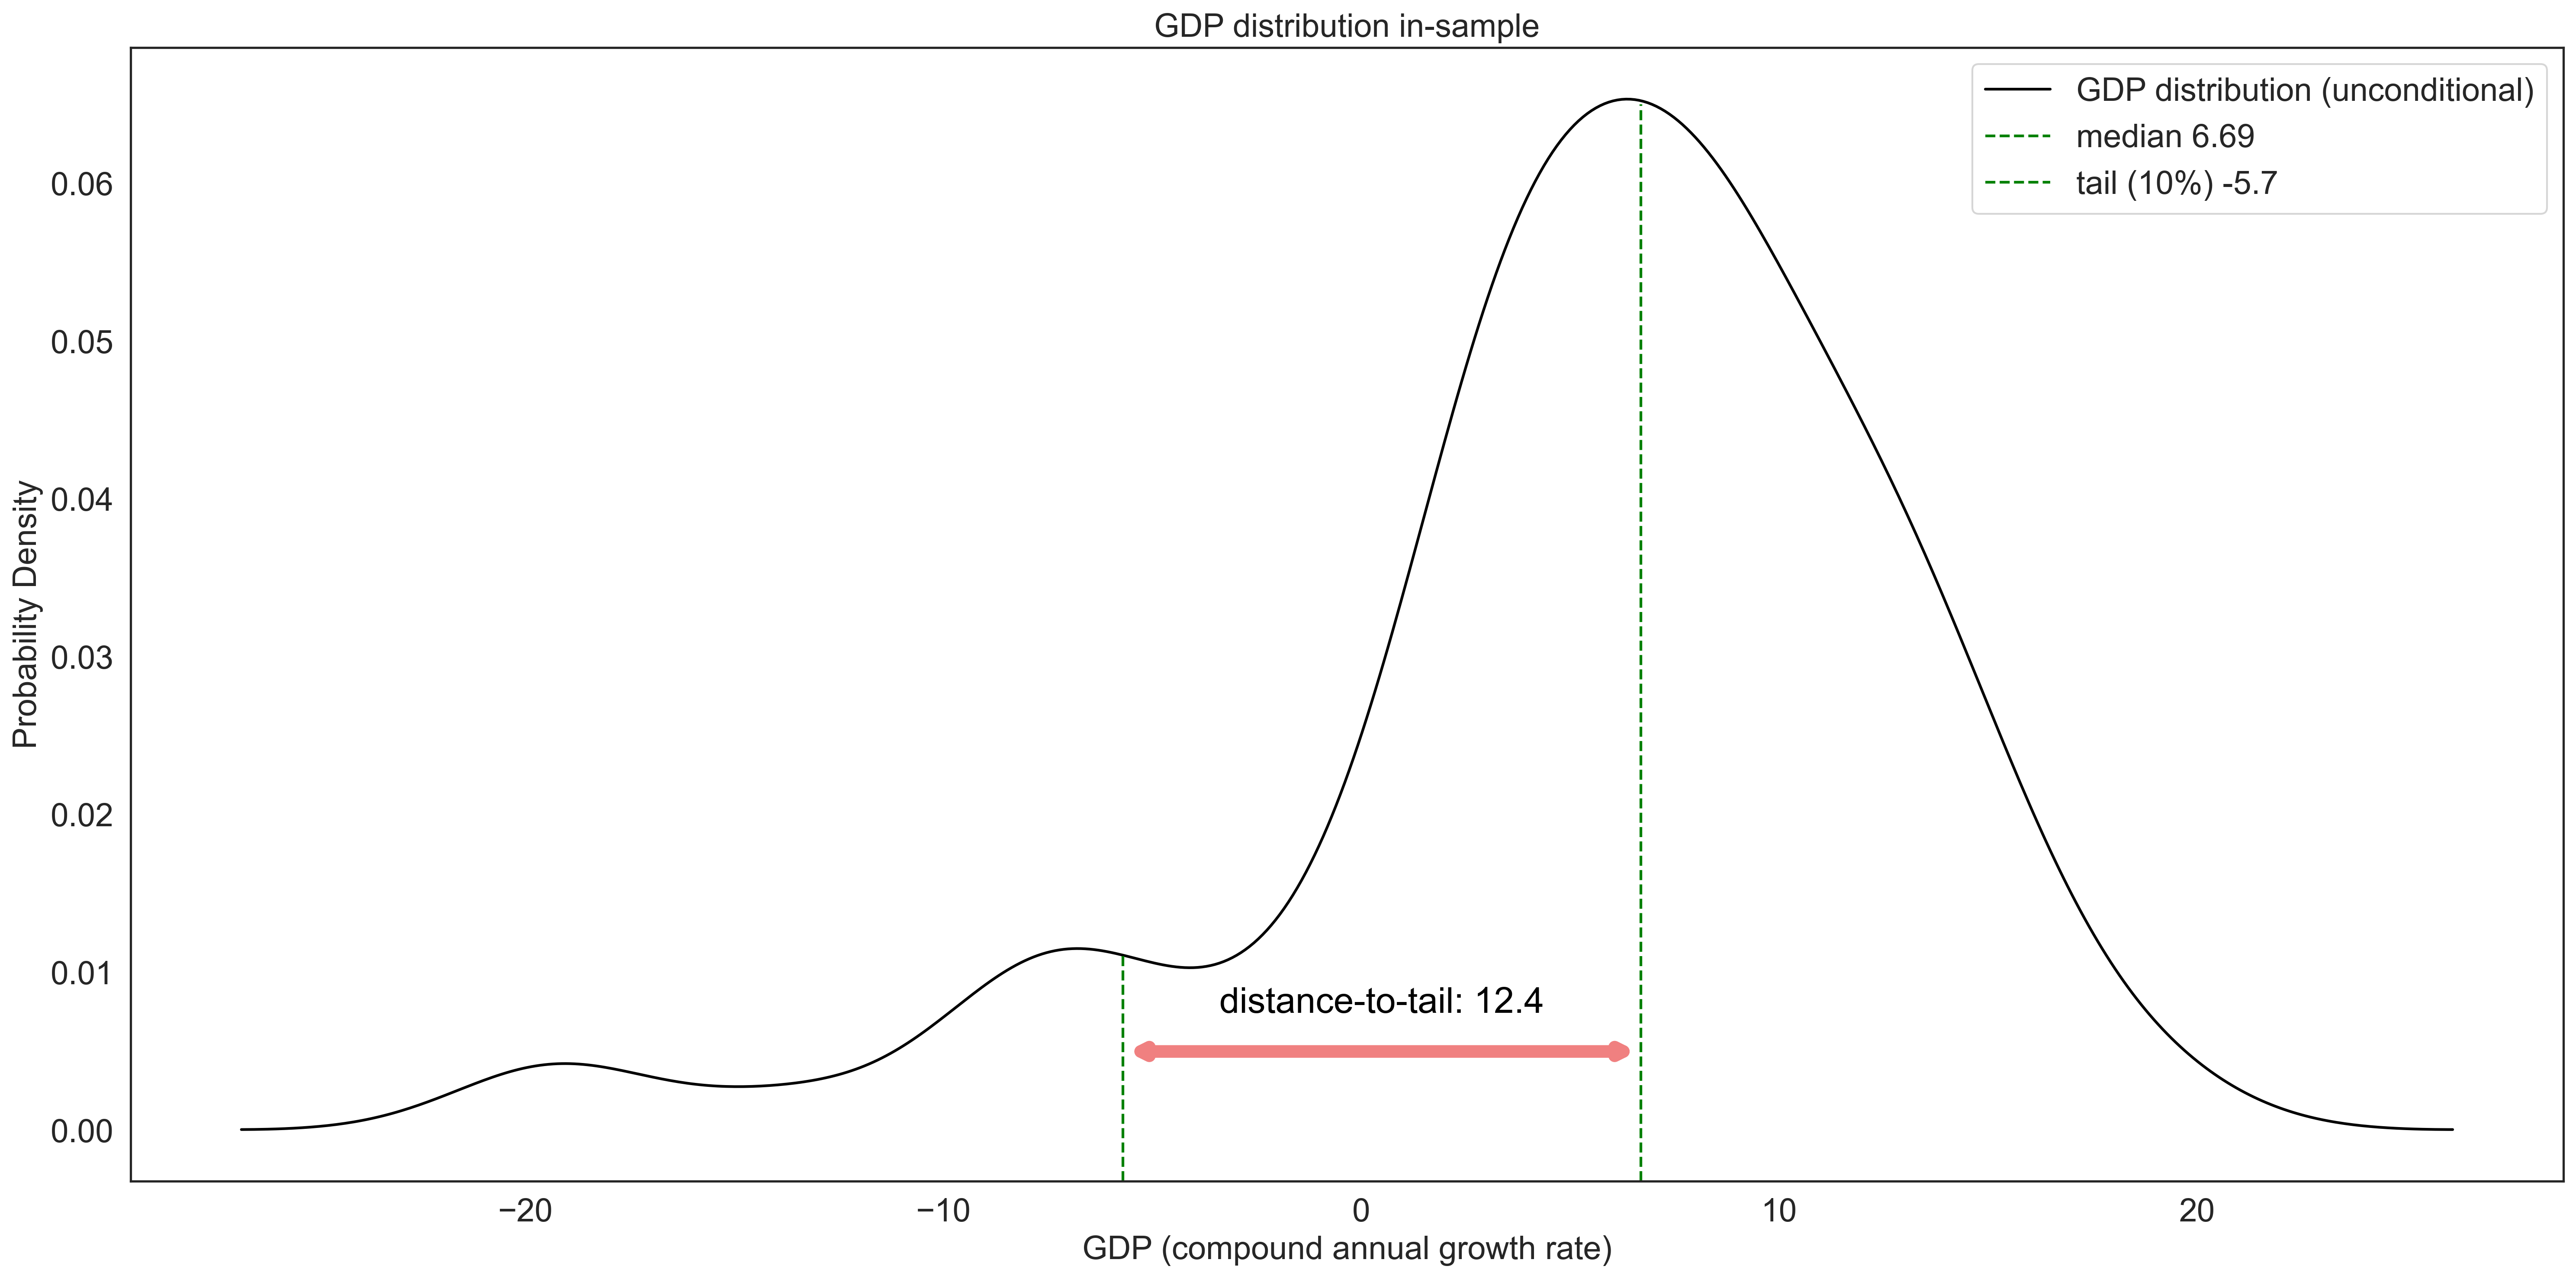
\includegraphics[width=0.45\textwidth, angle=0]{Figures/theory_gdp_unconditional.png}	
	\caption{Unconditional GDP growth distribution of Armenia and distance-to-tail.} 
	\label{fig:theory_gdp_unconditional}%
\end{figure}

In \autoref{fig:theory_policy}, we illustrate the GDP growth distribution of Armenia conditional on systemic risks. This conditional distribution displays how the risks shape the uncertainty surrounding GDP growth expectations. The conditional distance-to-tail serves as a means to quantify the negative impact that the buildup of systemic risks can exert on the economy. In the same figure, we simulate how a buildup of financial vulnerabilities, such as excessive credit growth a year prior will affect the shape of the distribution (shown in yellow). This type of environment may increase or decrease the median depending on the nature of externalities, but it will always negatively affect the tail. The distance-to-tail will sharply increase as a result, reflecting the potential severity of these risks. Lastly, we simulate the impact that a tightening of the macroprudential policy during excessive credit growth might have on the distribution (shown in green). While tightening policies tend to lower the median due to the short-term costs imposed on banks, they also improve the tail outcomes. As a result, the distance-to-tail decreases, signaling a reduction in negative outcomes related to systemic risks. This is both a result of the reduction in risks, but also the increased resilience of the system.
\begin{figure}
	\centering 
	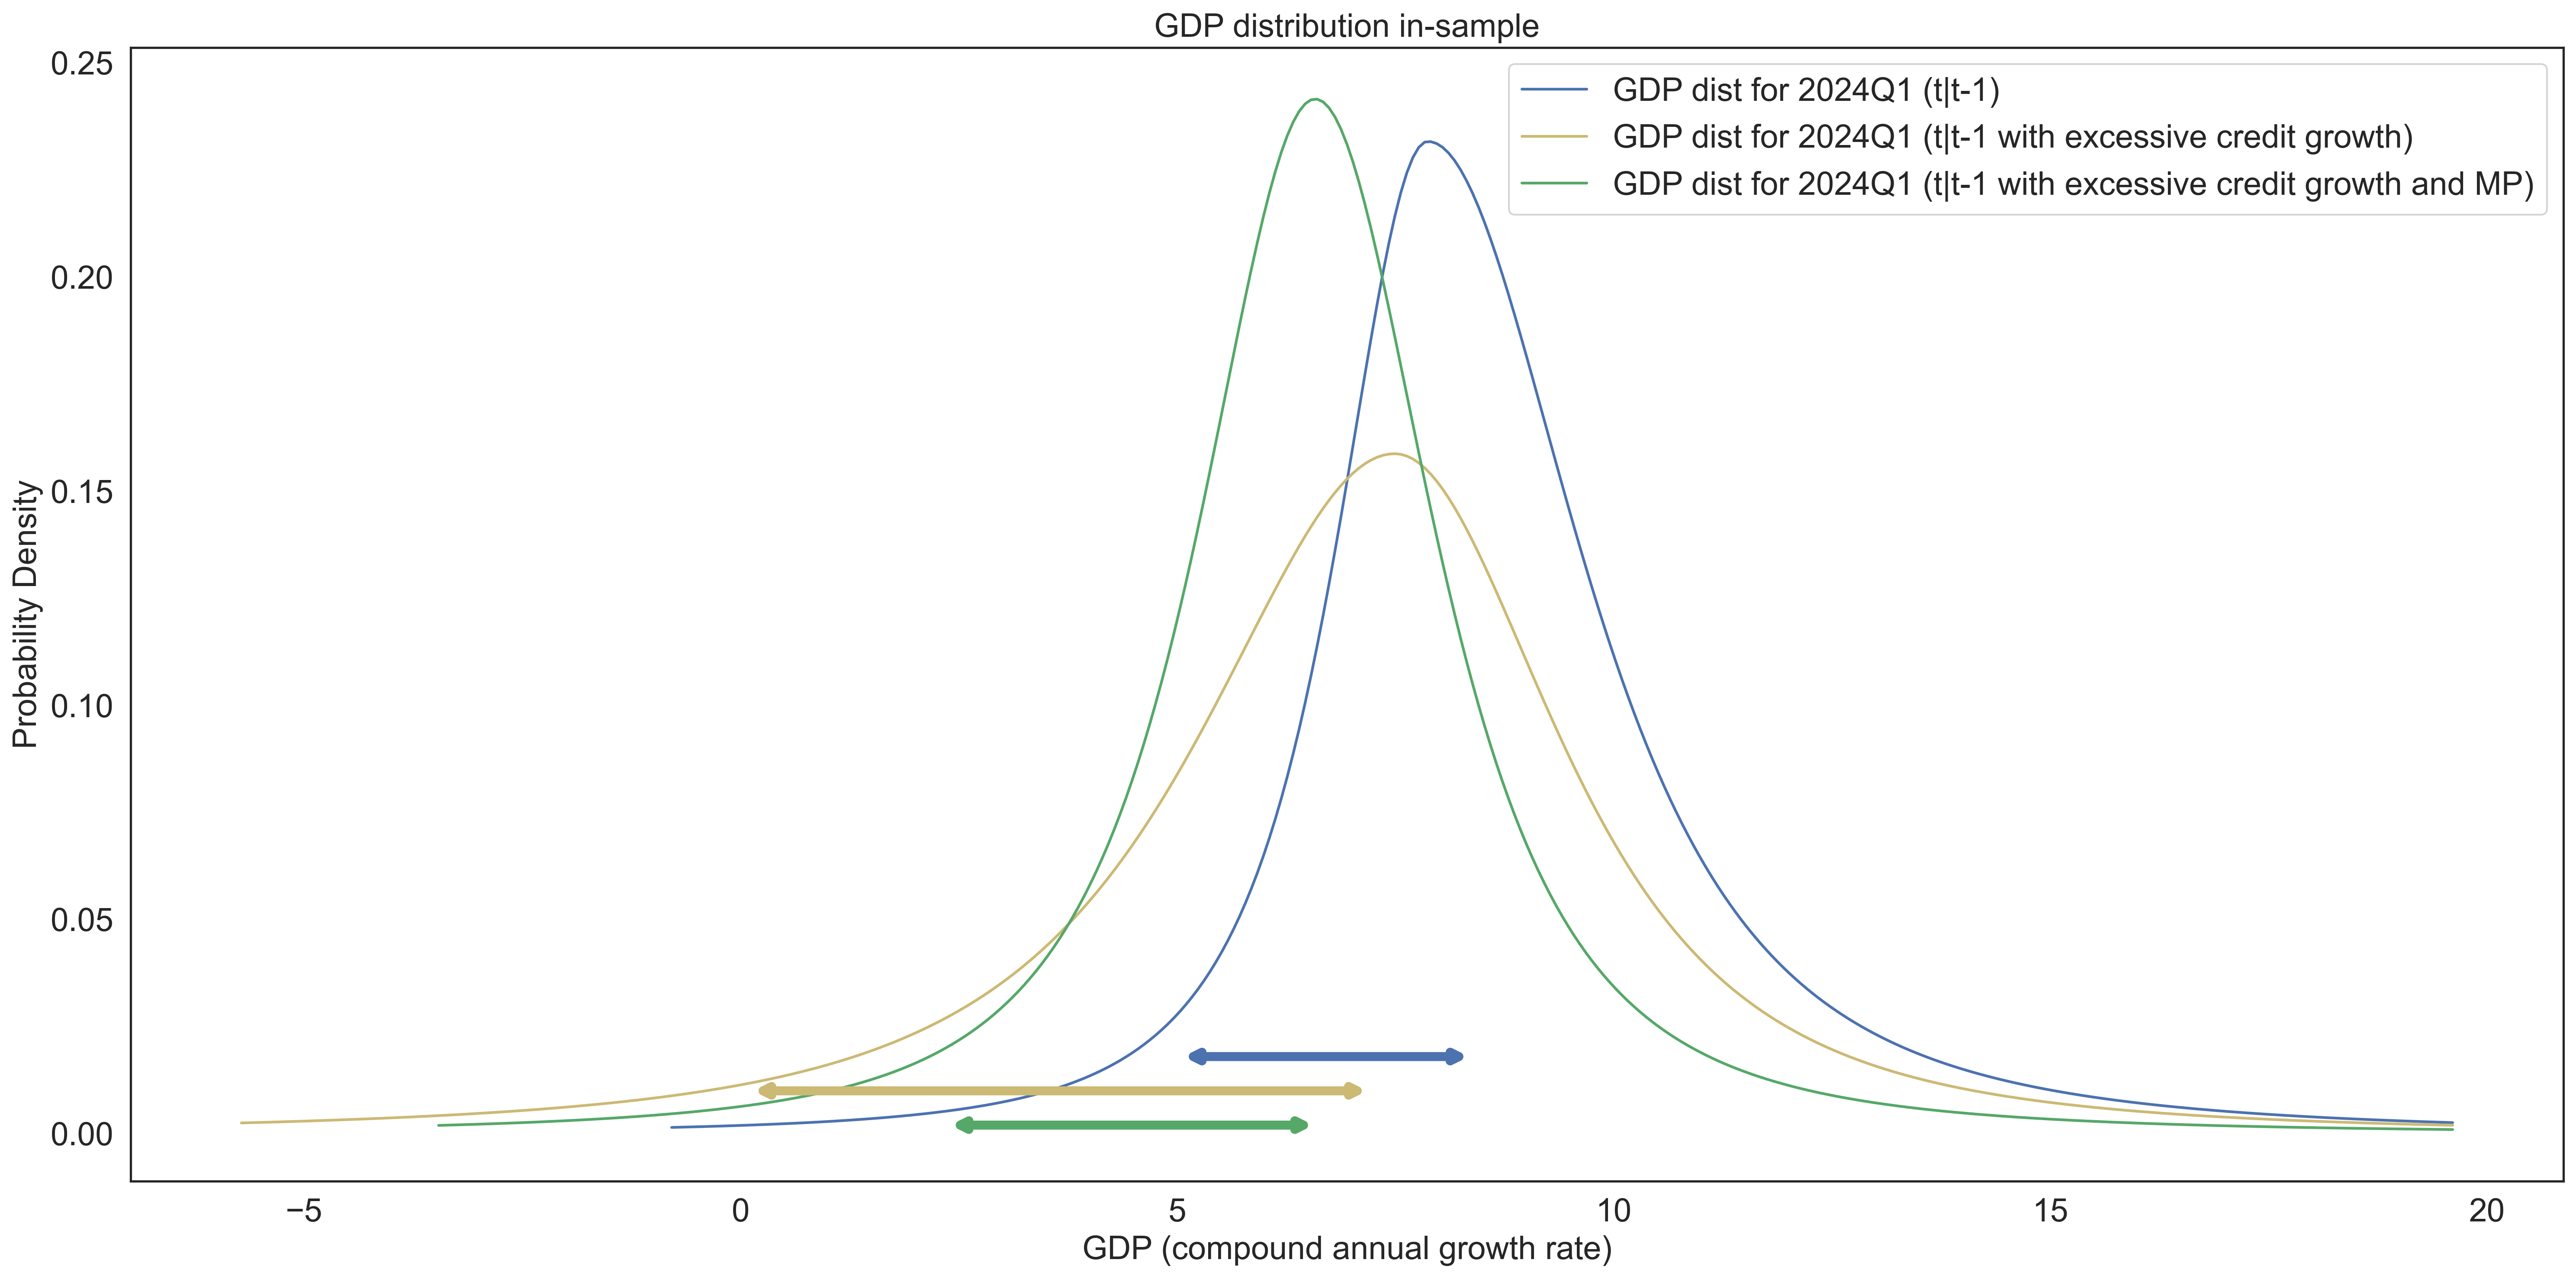
\includegraphics[width=0.45\textwidth, angle=0]{Figures/theory_policy.png}	
	\caption{GDP growth distribution of Armenia conditional on systemic risks in 2024Q1. The yellow distribution considers the effect of an increase in financial vulnerabilities, while the green distribution considers the former, but also a tightening of macroprudential policy.} 
	\label{fig:theory_policy}%
\end{figure}

\subsection{Macroprudential stance}
Generally, when considering macroprudential policy through the “risk-resilience framework,” a stance metric represents the residual systemic risk in the financial system \citep{esrb2019}. We derive the residual risk by “assessing the aggregate risk and subtracting any exogenous and/or policy-induced resilience” \citep{esrb2021}. From this perspective, macroprudential policy is a risk management approach, where we balance systemic risk and resilience while accounting for policymakers' tolerance of the net residual risk. As part of the indicator-based approach for Borrower-Based Measures (BBMs), \citet{esrb2024} defines the macroprudential stance as:
\begin{equation}
    \label{eq:stance}
    \textnormal{Stance} = \textnormal{Risk} - \textnormal{Resilience} - \textnormal{Policy}
\end{equation}

In the GaR framework, the conditional distance-to-tail tracks the changes in systemic risk over time, thus it can be used as one of the main indicators for the macroprudential stance. The metric primarily focuses on risks and policy, while using systemic thresholds as a reference for resilience. The systemic thresholds are calculated from the quantiles of the historical distance-to-tail series. The loss function for the distance-to-tail approach takes the form:
\begin{equation}
    \label{eq:dt_loss}
    \min_{\rho_t}\mathcal{L} = \max{\left((y_m - y_c), \textnormal{threshold}\right)}
\end{equation}

where $y_m$ and $y_c$ are the median and the tail, while ($y_m-y_c$) is the distance-to-tail. When this value exceeds the threshold, we are incentivized to tighten the macroprudential policy to minimize the loss. The complete \citet{esrb2024} formulation includes multiple thresholds at the 10th, 30th, 70th, and 90th percentiles of the distance-to-tail distribution. The resulting stances are classified into 5 categories: tight, grey-tight, neutral, grey-loose, and loose. Thus, the long-term goal of the policy is to maintain the stance at the neutral level.

The main limitation of this approach is that it does not consider the costs that macroprudential policy will impose for reducing systemic risks. Additionally, the systemic thresholds are not a dynamic measure of the resilience of the financial system. As an alternative to the distance-to-tail approach, we consider the welfare function proposed by \citet{suarez2022}. The function takes the form:
\begin{equation}
    \label{eq:suarez_W}
    W = y_m - \frac{1}{2}w\left(y_m - y_c\right)^2
\end{equation}
\begin{equation}
    \label{eq:suarez_loss}
    \min_{\rho_t}\mathcal{L} = -\mathop{\mathbb{E}_t}\left\{\sum_{t=0}^{T}\beta^tW_{t+1}\right\}
\end{equation}

where $w$ is interpreted as the aversion to financial instability, while $\beta$ is a discount factor. This formulation considers both the median and the distance-to-tail, capturing the costs of macroprudential policy along with its benefits \citep{cecchetti_2021}. It is apparent from \autoref{eq:suarez_W}, that the optimal policy is subject to the choice of $w\in(0,\inf)$. This term includes the policymakers’ appetite for risk, but also the probability of crisis. A higher value of w indicates that the policymaker is more sensitive to risks, while a value of zero would imply a complete disregard for the systemic risks in the economy. The calibration results indicate that the reasonable value of $w$ in Armenia is around 0.11\footnote{For detailed information on the calibration procedure, see \ref{appx:w_calibration}.}. The specific trade-off for the policymakers will depend on their tolerance for downside risks, but also the effectiveness of macroprudential policy \citep{esrb2021, suarez2022}.